\documentclass{standalone}
\usepackage{circuitikz}
\usepackage{siunitx}

%Start
\newcommand{\drawpulse}[2][0]{
    \begin{scope}[rotate=#1]
    \draw (#2.center) ++(-3mm, -2mm) -| ++(2mm,5mm)
    -- ++(2mm,0mm) |- ++(2mm, -5mm);
    \end{scope}
}
%End 

\begin{document}
    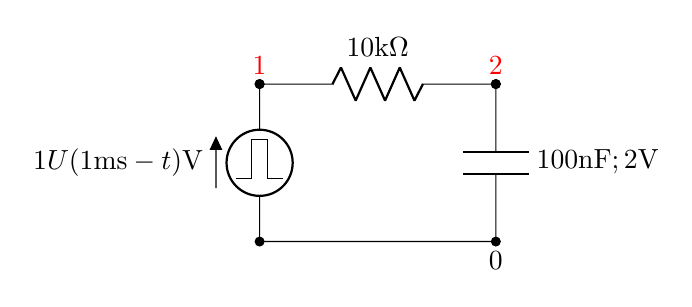
\begin{tikzpicture}
        \draw (0,0) to [esource, name=source, v=$1 U(1\si{\milli\second} - t)\si{\volt}$,*-*]++(0,2) node[label, above]{$\textcolor[rgb]{1.00,0.00,0.00}{1}$} to[R, label=$10\si{\kilo\ohm}$,*-*] ++(3,0) node[label, above]{$\textcolor[rgb]{1.00,0.00,0.00}{2}$} to[C, label=$100\si{\nano\farad}; 2\si{\volt}$,*-*] ++(0,-2)node[label, below]{$\textcolor[rgb]{0.00,0.00,0.00}{0}$} -| (source.west);
        \drawpulse{source}
    \end{tikzpicture}
\end{document}